\documentclass{article}
\usepackage{icomp2026_conference,times}
\usepackage{amsmath,amssymb,graphicx,booktabs,hyperref,url,etoolbox}
\hypersetup{hidelinks}
\makeatletter
\patchcmd{\@maketitle}{Paper under double-blind review}{Working manuscript; venue not selected}{}{\PackageError{draft}{Title patch failed}{Check template.}}
\makeatother
\title{Room for Doubt: Distilling Early Training Dynamics for Inference-Time Reliability}
\author{Anonymous authors}
\begin{document}
\maketitle
\lhead{Working draft --- 5 November 2026}
\begin{abstract}
A classifier's training dynamics can reveal how it learns from noisy
labels, but new images have no measured training history. We study two
ways to transfer early-training information to inference with frozen
ResNet50 features. The first predicts a class-conditioned probability
margin averaged over five early epochs and uses the predicted margin to
weight test-time augmentations. In exploratory experiments on three
independently trained bases per dataset, this scalar method gains 0.82
percentage points over uniform augmentation on CIFAR-100N and 1.07 on
CIFAR-10N Worse. The corresponding gains are 0.25 on Animal-10N and 0.75
on Mini-WebVision. Calibration does not consistently improve.

The second approach distills a five-checkpoint teacher into a one-pass
posterior head. On a prespecified CIFAR-10.1 test, residual distillation
changes accuracy by $-0.07$ percentage points against the base
(conditional paired 95\% interval $[-0.53, 0.42]$) and meets the latency
criterion. On CIFAR-10.2, the prespecified comparison of direct students
from the five-checkpoint and five-view teachers gives $-0.02$ points
($[-0.53, 0.48]$). In the secondary comparison the five-checkpoint teacher
itself gains 2.10 points over the five-view teacher. The exploratory
scalar results and the external tests characterize different uses of
early-training information. The tested one-pass heads did not meet
either prespecified primary accuracy criterion.

\end{abstract}
\section{Introduction}
A classifier trained with noisy annotations must learn useful visual structure while receiving incorrect supervision. Its final class probabilities summarize the selected model, but omit how its support for an annotation changed during learning. Training dynamics expose this information for examples encountered during optimization: dataset cartography describes confidence and variability, and margin-based ranking identifies potentially mislabeled examples \citep{swayamdipta2020dataset,pleiss2020identifying}. A deployment image, however, has no measured training trajectory.

We investigate a direct way to make part of this signal available at inference. A class-conditioned regressor learns an early-history summary from frozen image features and an observed annotation. At inference, the regressor takes the base model's predicted class as its conditioning label. Its output estimates the margin summary associated with that image--class pair. A monotone transformation of the output provides a reliability ranking and weights predictions across augmented views.

The central empirical question is whether the historical target contributes beyond learning a predictor of a static checkpoint statistic. We therefore keep the regressor architecture, feature dimension, training budget, and downstream weighting rule fixed when comparing an early-history mean, the mean over all recorded epochs, and a static margin. We separately compare features of the selected base classifier with an independent frozen ResNet18 encoder. This design distinguishes the target comparison from the effect of the feature source.

The evaluated early-history variant improves accuracy on both CIFAR-10N Worse and CIFAR-100N, with gains repeated on three independently trained CIFAR-100N bases and three CIFAR-10N Worse bases. The early summary outperforms the full-history mean in these exploratory CIFAR runs. The feature-source comparison also favors features from the selected base over those of the independent encoder for the early target. We report calibration and an ensemble baseline alongside these gains: an ensemble of two CIFAR-100N bases reaches higher accuracy than either base with the proposed weighting.

Our contribution is an empirical study of when early-training information
helps at inference under noisy supervision. We compare class-conditioned
scalar weighting with matched targets and evaluate posterior compression
in two prespecified external tests. CIFAR-10.1 measures residual
distillation against the original classifier. CIFAR-10.2 tests direct
distillation from five early checkpoints against one checkpoint with five
views. Neither test meets its prespecified primary accuracy criterion.
The latter experiment finds a teacher-level advantage that does not carry
over to the corresponding one-pass students. Independently trained bases
are the replication unit. Regressor initializations are nested within
each base.


\section{Related Work}
\paragraph{Training dynamics and annotation quality.}
Dataset cartography uses statistics collected throughout training to characterize examples \citep{swayamdipta2020dataset}. Area Under the Margin (AUM) ranks examples using accumulated logit margins \citep{pleiss2020identifying}. These methods motivate studying how a label is learned rather than relying on one checkpoint. Our targets are probability margins, so their scale and definition differ from AUM. We also predict a history summary for a new image, whereas the original training dynamics are observed only for the training samples.

DynaCor learns representations of training dynamics for noisy-label detection and introduces intentional label corruption to provide indirect supervision \citep{kim2024learning}. It is a close conceptual reference because it learns from temporal behavior instead of using a fixed hand-designed statistic alone. Our regression target is an observed-label margin summary, without intentional relabeling or clean/noisy detector supervision. The downstream evaluation concerns errors of the deployed classifier on clean test images. Detecting incorrect training annotations and detecting errors on unseen images are different events; performance on one is not evidence of performance on the other.

\paragraph{Learning with noisy labels.}
Generalized cross entropy changes the training objective to reduce sensitivity to noisy labels \citep{zhang2018generalized}. DivideMix models the distribution of training losses and uses semi-supervised learning with two networks \citep{li2020dividemix}. Our experiments use a cross-entropy warmup followed by generalized cross entropy as a fixed base-training recipe. Distillation is applied after this training and does not change its loss or remove examples. Combining the estimator with other robust-training methods is a separate empirical question. The present comparison measures inference changes on fixed bases rather than establishing a new accuracy benchmark against the best noisy-label training systems.

CIFAR-N provides human-annotated noisy training labels for CIFAR-10 and CIFAR-100 \citep{wei2022noisy}. This permits fitting with noisy labels while retaining clean labels for evaluation. We use the Worse annotation set for CIFAR-10N and the noisy fine-class annotations for CIFAR-100N. The availability of clean training annotations is not used to supervise the proposed regressor or select policies.

\paragraph{Reliability, calibration, and aggregation.}
Maximum softmax probability is a standard baseline for detecting prediction errors \citep{hendrycks2016baseline}. Calibration asks whether confidence agrees with empirical correctness, a distinct property from ranking errors \citep{guo2017calibration}. We therefore report error-detection AUROC and calibration metrics separately. The proposed badness score is a bounded ranking score, not a calibrated posterior probability of noise or error.

Deep ensembles average predictions of independently trained models \citep{lakshminarayanan2017simple}. They are relevant both as a reliability baseline and as an alternative use of additional training compute. Test-time augmentation instead averages predictions across transformed versions of an image. Learned aggregation has already been studied directly \citep{shanmugam2021aggregation}; weighting views itself is not the novelty here. Our question is whether a distilled temporal target supplies a useful view score under noisy supervision. Uniform, maximum-probability, probability-gap, and entropy weighting share the same cached views in our evaluation. A learned aggregation baseline under the same supervision and compute budget remains a relevant comparison.


\paragraph{Snapshot distillation and fixed features.}
Snapshot Distillation uses earlier weights as teachers during later
cycles of the same training run~\citep{yang2019snapshot}. Jeong and Chung
study self-distillation under label noise with fixed feature extractors
and use the teacher's top predictions for partial-label
refinement~\citep{jeong2025rethinking}. ELDET uses early teachers to address
categorization and localization noise in object detection~\citep{choi2025eldet}.
Our posterior experiments hold the trained classifier and head budget
fixed. They compare averaging early checkpoints with averaging views
from one checkpoint. These studies provide context for the design. The
reported controls do not reproduce their full training procedures.

\section{Method}
\label{sec:method}
Let $\mathcal D_{\mathrm{train}}=\{(x_i,\tilde y_i)\}$ contain images and observed, potentially incorrect labels. A base classifier produces class probabilities $p_{\theta}(c\mid x)$. We select a checkpoint $\theta^*$ using noisy-validation cross entropy and freeze it for the remaining stages.

\paragraph{Observed-label history.}
For each training example we record one probability margin per epoch:
\begin{equation}
 m_{it}=p_{\theta_{it}}(\tilde y_i\mid a_{it}(x_i))-
 \max_{c\ne\tilde y_i}p_{\theta_{it}}(c\mid a_{it}(x_i)),\qquad m_{it}\in[-1,1].
\end{equation}
Here $a_{it}$ is the training augmentation and $\theta_{it}$ denotes the weights at that example's minibatch forward pass, before its update. Thus an epoch's margins are not evaluated at one common epoch-end checkpoint. The primary scalar target is
\begin{equation}
 s_i^{(K)}=\frac1K\sum_{t=1}^{K}m_{it},\qquad K=5.
\end{equation}
All reported bases were trained for 50 epochs. Using the first five recorded margins does not imply that the base itself was trained for only five epochs.

\paragraph{Class-conditioned regression.}
Let $h_{\theta^*}(x)\in\mathbb R^{2048}$ be the base's penultimate feature vector. We fit a centered, non-whitened principal-component projection $P$ on meta-training images only and retain 512 dimensions. The estimator concatenates the projected features with a learned 32-dimensional class embedding:
\begin{equation}
 \hat s(x,c)=g_{\phi}\big(P(h_{\theta^*}(x)-\mu),e(c)\big).
\end{equation}
The regressor has a 256-unit ReLU hidden layer and a scalar linear output. It minimizes mean squared error between $\hat s(x_i,\tilde y_i)$ and $s_i^{(K)}$. Its checkpoint minimizes held-out meta-validation MSE. Each training image contributes its observed class only; there is no supervision for all possible candidate classes. At deployment we substitute the base's predicted class, which introduces a conditioning shift evaluated empirically.

\paragraph{Reliability score and weighted views.}
For a view $v$ of a test image, let $c_v=\arg\max_c p_{\theta^*}(c\mid v)$. We define
\begin{equation}
 B(v)=\operatorname{clip}\left(\frac{1-\hat s(v,c_v)}2,0,1\right),\quad
 w_v=\frac{\exp(-B(v)/T)}{\sum_{u=1}^{V}\exp(-B(u)/T)},\quad
 \bar p=\sum_{v=1}^{V}w_vp_{\theta^*}(\cdot\mid v).
\end{equation}
The predicted label is $\arg\max_c\bar p_c$. Higher badness indicates a smaller predicted historical margin; it is not a probability of memorization. The selected base features can be reused from the classifier's forward pass. Each view still requires a base-model evaluation, a projection, and a regressor evaluation. Uniform weighting is included as an exact alternative, rather than only approximated by a large temperature.

\paragraph{Matched controls.}
The static target is the observed-label probability margin of the selected checkpoint on the unaugmented training image. History-50 averages all 50 recorded margins. Both targets use the same scalar head, initialization seed, loss, training budget, and policy search as Early-5. A second feature condition uses frozen ImageNet ResNet18 features, also projected to 512 dimensions with train-only PCA. Comparisons within a feature condition hold the head fixed while changing target construction. Temporal and static targets also differ in augmentation and online versus evaluation-time measurement, so this is not a causal isolation of temporal information. Comparisons between feature conditions assess the representation source. The primary method uses neither a clean/noisy supervised detector nor Top-2 overrides.


\section{Experimental Protocol}
\label{sec:protocol}
\paragraph{Data and base training.}
Each CIFAR dataset has 50,000 training images and 10,000 clean test images. A fixed seed-42 shuffle divides training images into 45,000 noisy-training and 5,000 noisy-validation samples. Base initialization seeds vary while membership in these sets stays fixed. ResNet50 starts from torchvision ImageNet-1K V2 weights, with inputs resized to $224\times224$. We train for 50 epochs using SGD (learning rate 0.01, momentum 0.9, weight decay $5\times10^{-4}$), cosine annealing, and a global batch size of 128. Base training uses mixed precision on two Tesla T4 GPUs through data parallelism. The first five epochs use cross entropy and later epochs use generalized cross entropy with $q=0.7$. The checkpoint with minimum noisy-validation cross entropy is selected. It is epoch 2 (one-based) for CIFAR-100N seeds 42/43 and CIFAR-10N seeds 42/43/44, and epoch 3 for CIFAR-100N seed 44. All selected checkpoints are within the cross-entropy warmup.

\paragraph{Meta-training and selection.}
For CIFAR, a fixed shuffle with seed 20261015 partitions the 45,000 base-training IDs into 27,000 meta-training, 4,499 meta-validation, 6,751 reserved detector-fit, and 6,750 diagnostic-evaluation IDs. The one-example deviation from a 60/10/15/15 split reflects integer truncation in the saved implementation. The detector-fit partition is unused by this estimator. PCA and regression use only meta-training IDs; the regression checkpoint uses meta-validation targets. These images were nevertheless seen during base training, so held-out regression diagnostics are not equivalent to evaluation on images unseen by the base.

Heads are trained for 25 epochs with Adam, learning rate $10^{-3}$ and batch size 256, using initialization seeds 42, 43, and 44. The two feature sources and all target controls have matched input dimension and head architecture. Clean training labels are accessed only in post-selection annotation-noise diagnostics, not in fitting, descriptor construction, or model selection.

\paragraph{View and temperature selection.}
A shared deterministic stream supplies the original image followed by reflected-padding random crops and horizontal flips at the original CIFAR resolution; each view is then resized and normalized. We search $V\in\{1,5,10\}$ and $T\in\{0.02,0.05,0.1,0.25,0.5,1,2,5,10,10^6\}$ plus exact uniform weighting. Selection maximizes accuracy on the noisy-validation labels. Ties prefer fewer views, then uniform weighting. Each head has its own selected policy; the selected policy table is saved before that run's test evaluation. Base checkpoint and policy selection reuse the same noisy-validation set. This is validation reuse, not an additional independent validation sample.

\paragraph{Metrics and statistical units.}
Accuracy, negative log likelihood (NLL), multiclass Brier score, and expected calibration error (ECE; 15 equal-width confidence bins) are computed from each method's final probabilities. Error AUROC ranks the fixed original-view base errors using the corresponding original-view score; it is not the AUROC of the errors remaining after TTA. The three head-seed results are averaged within each independently trained base. Reported standard deviations describe head initialization only. Paired accuracy intervals use 2,000 multinomial bootstrap draws over test-example correctness differences and the 2.5/97.5 percentiles. They are nominal intervals conditional on the fitted models and policies, without a multiple-comparison correction.

\paragraph{Exploratory scope.}
The completed evidence contains three CIFAR-100N bases (seeds 42, 43, 44) and three CIFAR-10N Worse bases (seeds 42, 43, 44). CIFAR-10N seed 44, initially deferred by the campaign admission rule, is now complete under the same recipe. The CIFAR-10N base-42 follow-up rebuilds the standard 18-head feature study on the original verified checkpoint; all 23 original selected-policy accuracies, view counts and temperatures reproduce. This is a reconstruction on the same base, not an additional independent base run. The test benchmarks have been inspected during method development. Early-5 was selected as the primary target after an initial window study and carried forward into the subsequent runs; this is not a preregistered, untouched-test confirmation. Table entries use FP32 downstream evaluation consistently. The AMP evaluations exported by base training differ from downstream FP32 accuracy by 0.01--0.05 percentage points across these runs and are not mixed into downstream gains. Dataset summaries first average the three heads within each base, then weight independent bases equally; their sample standard deviations describe between-base gain variation, not confidence intervals.


\section{Results}
\paragraph{Accuracy on independently fitted bases.}
Table~\ref{tab:accuracy} compares policies selected on noisy validation; Figure~\ref{fig:accuracy_gain} shows gains relative to each base. Early-5 with base features raises CIFAR-100N accuracy from 70.12\% to 71.08\% (base 42), 69.23\% to 70.28\% (base 43), and 69.57\% to 70.09\% (base 44). On CIFAR-10N Worse, accuracy rises from 88.84\% to 90.16\% (base 42) and 89.63\% to 91.28\% (base 43). Gains are positive for the head mean on all five bases. However, the nominal paired interval for CIFAR-100N base 44, head 43 is $[-0.19,+0.82]$ points relative to its base, and includes zero (Appendix~\ref{app:intervals}). Positive intervals against same-view TTA need not imply positive intervals against the globally selected TTA policy.

Averaging heads within each base and then independent bases equally, CIFAR-100N accuracy changes from 69.64\% to 70.48\%, a mean gain of 0.84 points (between-base sample SD 0.28; $n=3$ bases). CIFAR-10N Worse changes from 89.24\% to 90.72\%, a gain of 1.49 points (sample SD 0.23; $n=2$ bases). Mean gains over validation-selected uniform TTA are 0.82 points on each dataset. These small replication counts do not establish a universal effect or a precise population-level gain.
\begin{table}[t]
\centering\small
\caption{Test accuracy (\%). Columns identify base seeds within each dataset panel. Mean $\pm$ sample standard deviation is over three head initializations on the same base; non-learned weighting scores have no head-seed variation. Each method selects its own view budget and temperature on noisy validation.}
\label{tab:accuracy}
\begin{tabular}{lrrr}
\toprule
Method / dataset & \multicolumn{3}{c}{Base initialization} \\
\midrule
\multicolumn{4}{l}{\textbf{CIFAR-100N}} \\
Method & Base 42 & Base 43 & Base 44 \\
Base & 70.12 & 69.23 & 69.57 \\
Uniform TTA & 70.15 & 69.26 & 69.57 \\
MSP weighting & 70.15 & 69.26 & 69.57 \\
Gap weighting & 70.15 & 69.23 & 69.57 \\
Entropy weighting & 70.15 & 69.26 & 69.57 \\
Early-5, ResNet18 & 70.41 $\pm$ 0.12 & 69.32 $\pm$ 0.09 & 69.33 $\pm$ 0.13 \\
Static, base features & 70.35 $\pm$ 0.10 & 69.27 $\pm$ 0.01 & 69.57 $\pm$ 0.00 \\
History-50, base features & 70.46 $\pm$ 0.18 & 69.93 $\pm$ 0.09 & 69.68 $\pm$ 0.18 \\
Early-5, base features & 71.08 $\pm$ 0.24 & 70.28 $\pm$ 0.13 & 70.09 $\pm$ 0.21 \\
\multicolumn{4}{l}{\textbf{CIFAR-10N Worse}} \\
Method & Base 42 & Base 43 & Base 44 \\
Base & 88.84 & 89.63 & 88.49 \\
Uniform TTA & 89.29 & 90.52 & 88.82 \\
MSP weighting & 89.27 & 90.51 & 88.57 \\
Gap weighting & 89.27 & 90.58 & 88.82 \\
Entropy weighting & 89.30 & 90.53 & 88.82 \\
Early-5, ResNet18 & 90.01 $\pm$ 0.17 & 90.77 $\pm$ 0.23 & 89.34 $\pm$ 0.06 \\
Static, base features & 89.19 $\pm$ 0.13 & 90.53 $\pm$ 0.02 & 88.82 $\pm$ 0.10 \\
History-50, base features & 89.01 $\pm$ 0.31 & 90.43 $\pm$ 0.12 & 89.35 $\pm$ 0.19 \\
Early-5, base features & 90.16 $\pm$ 0.02 & 91.28 $\pm$ 0.02 & 90.39 $\pm$ 0.15 \\
\bottomrule
\end{tabular}

\end{table}

\begin{figure}[t]
\centering
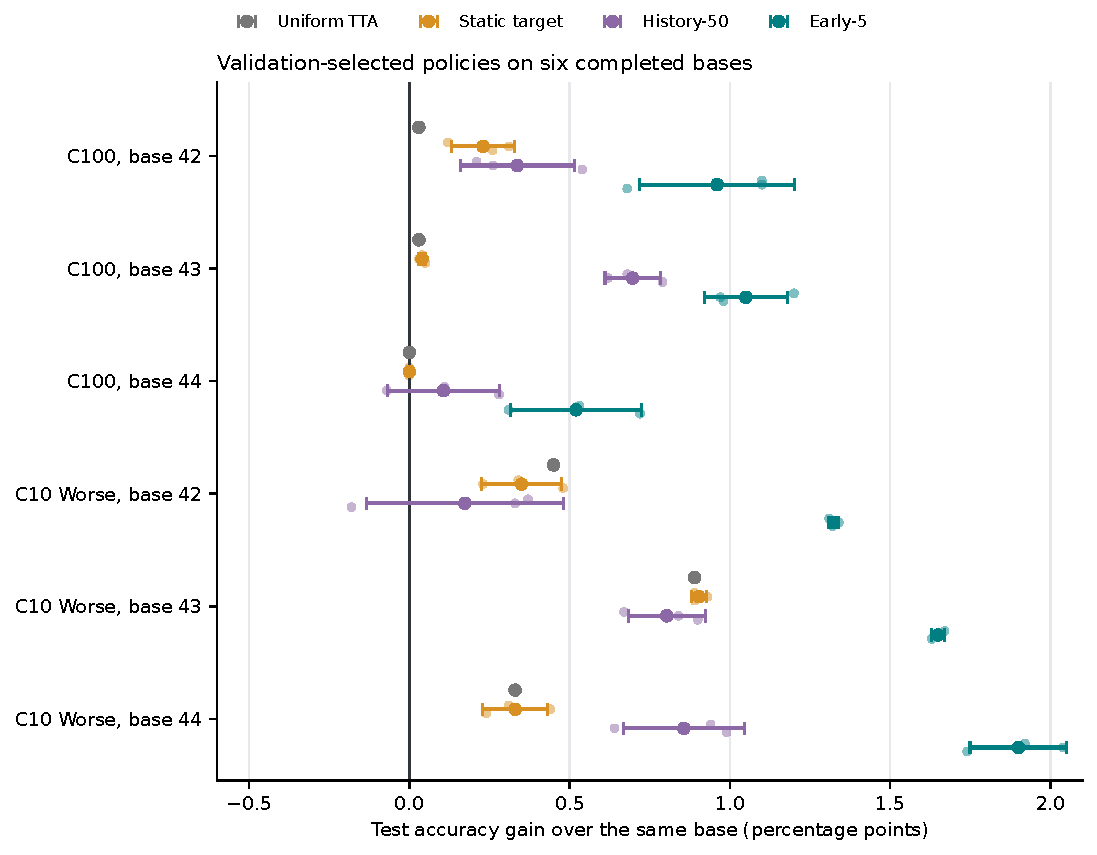
\includegraphics[width=\linewidth]{figures/accuracy_gain.pdf}
\caption{Accuracy gain over each corresponding base. Large dots and bars show the mean and sample standard deviation across three head seeds; small dots show individual heads. Bars do not estimate base-training uncertainty. Uniform TTA has no head. Each method selects its own view count and temperature on noisy validation.}
\label{fig:accuracy_gain}
\end{figure}

\paragraph{Target construction with matched heads.}
With base features, static-margin regression obtains 70.35\%, 69.27\%, and 69.57\% for CIFAR-100N bases 42/43/44, and 89.19\% and 90.53\% for CIFAR-10N Worse bases 42/43. Early-5 is higher in each case with the same head architecture and policy-search procedure; the History-50 mean is also lower than Early-5 on each base. The difference is therefore not explained solely by adding a trainable scalar head. It does not distinguish temporal information from the different augmentation and measurement conditions used to construct the targets. These are comparisons of the complete validation-selected policies; their selected temperatures and sometimes view budgets differ. Direct paired target comparisons are now available for CIFAR-100N base 44 and CIFAR-10N Worse base 43 (Appendix~\ref{app:followup_controls}); comparisons on the other three bases remain point estimates.

\paragraph{Augmentation-matched static control.}
On CIFAR-100N base 44 and CIFAR-10N Worse base 43, a follow-up static target averages five new deterministic draws from the actual training augmentation distribution at the fixed selected checkpoint. It uses the same frozen base features, train-only PCA, head architecture, three head seeds and 25-epoch budget. The previous nine base-feature heads per base are reused, and only three augmented-static heads are fitted. Policies are selected on noisy validation before test evaluation. This matches the augmentation distribution, not the unrecorded original RNG draws or changing online weights.

Augmented-static weighting obtains 69.57\% versus Early-5's 70.09\% on CIFAR-100N, and 90.61\% versus 91.28\% on CIFAR-10N Worse. The latter static control improves over the original static target's 90.53\%, but leaves a 0.67-point Early-5 advantage. On CIFAR-100N the gap is 0.52 points; augmented-static selects one view for each head, while Early-5 selects five or ten. For CIFAR-10N, all three nominal paired Early-5 minus augmented-static accuracy intervals are strictly positive. For CIFAR-100N, two of three include zero (one has lower endpoint exactly zero). Original-view AUROC difference intervals are positive for all six heads. These conditional comparisons strengthen the evidence beyond the original static control, while not isolating time from weight evolution, checkpoint timing or the CE/GCE schedule. Full results and policy budgets appear in Appendix~\ref{app:followup_controls}.

\paragraph{Early summaries and feature sources.}
The initial CIFAR-100N seed-42 window study is reported in Table~\ref{tab:windows} and Figure~\ref{fig:history_windows}. The first ten epochs give the highest observed test accuracy in that sweep, while the last five epochs and the full-history mean are weaker. This sweep is exploratory and does not select an optimal window using test accuracy. The primary Early-5 target also coincides with the cross-entropy warmup; later epochs use a different loss. Thus the window effect combines learning time and the loss schedule.

For Early-5, replacing ResNet18 features with selected-base features changes accuracy from 70.41\% to 71.08\% on CIFAR-100N seed 42, from 69.32\% to 70.28\% on seed 43, and from 90.01\% to 90.16\% on CIFAR-10N seed 42. The full five-base comparison, including the new ResNet18 controls, appears in Table~\ref{tab:accuracy}. Both encoders are fixed during head training, but their pretraining and task adaptation differ. This comparison supports using the selected base representation under this recipe; it does not isolate encoder architecture from adaptation.
\begin{table}[t]
\centering\small
\caption{Exploratory history-window study on CIFAR-100N, base seed 42. Accuracy is in percent; AUROC detects original-view base errors. Entries average three head seeds. All targets use scalar regression.}
\label{tab:windows}
\begin{tabular}{lrrrr}
\toprule
Target & R18 acc. & R18 AUROC & Base acc. & Base AUROC \\
\midrule
First 2 & 70.20 & 0.7391 & 70.88 & 0.8053 \\
First 5 & 70.41 & 0.7472 & 71.08 & 0.8307 \\
First 10 & 70.33 & 0.7414 & 71.25 & 0.8330 \\
First 20 & 70.26 & 0.7164 & 70.98 & 0.7920 \\
All 50 & 70.28 & 0.6599 & 70.46 & 0.7112 \\
Last 5 & 70.19 & 0.5641 & 70.23 & 0.5932 \\
Static checkpoint & 70.16 & 0.7021 & 70.35 & 0.8045 \\
\bottomrule
\end{tabular}

\end{table}

\begin{figure}[t]
\centering
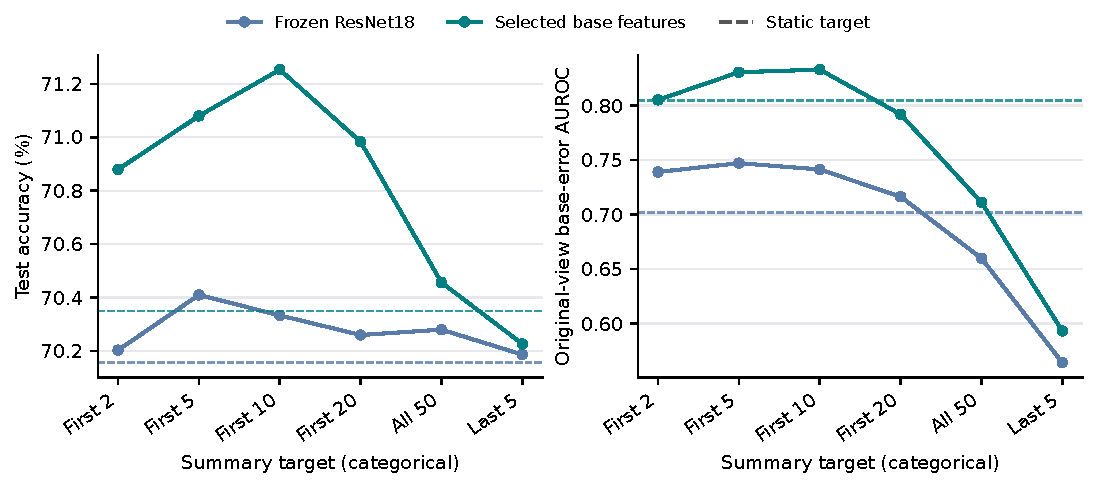
\includegraphics[width=\linewidth]{figures/history_windows.pdf}
\caption{Exploratory targets on CIFAR-100N, base seed 42. Points average three heads. Dashed lines show the static target for each feature source. Horizontal positions are categorical, not an epoch-time axis. Early-5 coincides with the cross-entropy warmup; the figure does not isolate learning time from the loss schedule or checkpoint timing.}
\label{fig:history_windows}
\end{figure}

\paragraph{Error ranking and calibration.}
Early-5 with base features increases original-view error AUROC on all five bases. For CIFAR-100N bases 42/43/44, MSP-to-Early-5 values are 0.8124 to 0.8307, 0.8222 to 0.8326, and 0.8281 to 0.8325. For CIFAR-10N Worse bases 42/43 they are 0.8764 to 0.9064 and 0.8758 to 0.8976. These rankings are separate from the gains in aggregated prediction accuracy.

CIFAR-10N calibration is metric- and base-dependent: ECE changes from 0.2847 to 0.2756 on base 42, but from 0.2518 to 0.2542 on base 43. NLL improves on both (0.6203 to 0.5903; 0.5591 to 0.5359). On all three CIFAR-100N bases, Early-5 worsens both ECE and NLL relative to the original-view base. Better accuracy or error ranking therefore does not imply improved probability calibration. Full results appear in Appendix~\ref{app:calibration}.

\paragraph{Ensembles and computational cost.}
A fixed original-view average of CIFAR-100N bases 42 and 43 reaches 73.01\%, exceeding either base with Early-5 weighting. This is the previously completed two-base ensemble; no new three-base ensemble is reported. Its nominal paired gain over base 42 is 2.89 points, with interval $[2.32,3.50]$. The comparison uses a different inference budget: the ensemble evaluates two bases once each, whereas the selected Early-5 policies evaluate one base on five or ten views depending on base and head. Globally selected uniform TTA uses ten views on four bases, but one view on CIFAR-100N base 44. There is therefore no demonstrated latency or forward-pass advantage over this two-base ensemble. Relative to uniform TTA at the same number of views, base-feature reuse avoids a second image encoder but adds PCA and the head.

Training cost includes the 50-epoch base run, trajectory recording, feature extraction, PCA, and head fitting. The experiments fit multiple controls and head seeds, so campaign wall time is not the cost of fitting a single deployment head. Storage for 45,000 float32 margins over 50 epochs alone is 9 MB in decimal units; cached features, weights, and predictions add further storage. The head contains $139{,}777+32C$ trainable parameters for $C$ classes. Training-overhead measurements remain needed to quantify the full tradeoff. A completed T4 inference microbenchmark is reported in Appendix~\ref{app:runtime}: for one image and five views on CIFAR-100N base 44, medians including CPU preprocessing and transfer are 20.25 ms for uniform TTA and 20.36 ms for Early-5. For ten views on CIFAR-10N base 43 they are 40.93 and 41.01 ms. Corresponding one-view base measurements are 7.59 and 7.52 ms. Thus the observed incremental head cost is small relative to matched-view TTA, while multi-view inference remains more expensive than one base pass. One session and fixed timing order do not establish statistical equivalence of these close medians or an advantage over an ensemble.


\section{Animal-10N transfer and independent replications}
\label{sec:animalpilot}
The Animal-10N experiment transfers the CIFAR recipe without tuning it to Animal test outcomes. Base 42 was the technical pilot; bases 43 and 44 were planned before fitting the pilot and were subsequently run with the same settings regardless of the pilot's favorable sign. All three runs retain the frozen protocol file byte-for-byte, 50 training epochs, a fixed 45,000/5,000 observed-label train/validation partition, three nested head seeds, and unchanged target and policy grids. The minimum noisy-validation cross entropy occurs at zero-based epochs 2, 1, and 2 respectively. Thus the experiment contains three independently initialized bases, not nine base replications or three independently resampled dataset splits.

The data realization is an explicitly identified public Activeloop mirror of Animal-10N~\citep{song2019selfie}, with 50,000 training and 5,000 test RGB $64\times64$ images. Repacking preserves decoded pixels, stored labels and train/test membership; IDs follow mirror row order. Original KAIST IDs/order and equality to the original archive are not independently verified. All runs record the same supplied-file hashes and saved source provenance. Complete clean training labels are unavailable; training-noise detection metrics are not reported.

\begin{table}[t]
\centering
\small
\begin{tabular}{lrrrrr}
\toprule
Method & Base42 & Base43 & Base44 & Mean & Error AUROC \\
\midrule
Base FP32 & 89.24 & 88.80 & 89.18 & 89.07 & 0.9079 \\
Uniform TTA & 89.56 & 89.86 & 89.92 & 89.78 & 0.9079 \\
MSP & 89.82 & 89.88 & 89.82 & 89.84 & 0.9079 \\
Static & 89.61 & 89.96 & 89.92 & 89.83 & 0.8954 \\
Augmented static & 89.68 & 89.89 & 89.92 & 89.83 & 0.8927 \\
History-50 & 89.95 & 90.22 & 89.91 & 90.03 & 0.8202 \\
Early-5 & 90.11 & 90.01 & 89.96 & 90.03 & 0.9091 \\
\bottomrule
\end{tabular}

\caption{Animal-10N accuracy (\%) by independent base and equal-base mean, followed by mean original-view base-error AUROC. Learned rows first average three heads within each base. Every method selects its own budget and temperature on noisy validation.}
\label{tab:animalpilot}
\end{table}

\paragraph{Accuracy gains attenuate in replication.}
Early-5 obtains 90.03\% averaged equally over bases, compared with 89.07\% for the matched downstream FP32 bases and 89.78\% for selected uniform TTA. The mean gains are 0.96 and0.25 percentage points. The TTA advantage by base is 0.55, 0.15, and 0.04 points; its between-base sample SD is0.27 points, not a confidence interval. Five of nine nominal conditional head-level paired intervals against selected TTA strictly exclude zero. One Early-5 head on base 43 is below TTA in point accuracy. These results preserve a positive within-base mean in each run but show a weaker and less consistent effect than the first pilot alone suggested.

\paragraph{Static and full-history controls.}
The augmentation-matched static control averages 89.83\%, a 0.20-point mean Early-5 advantage. Only two of nine conditional accuracy intervals strictly exclude zero, one touches zero and six cross zero. All nine corresponding original-view error-AUROC difference intervals are positive. History-50 averages 90.0267\%, versus 90.0289\% for Early-5: their 0.0022-point difference is negligible at the displayed precision. No paired Early-5 accuracy interval against History-50 is strictly positive; one on base 43 strictly favors History-50 and eight cross zero. Consequently the transfer results do not establish a general accuracy advantage of Early-5 over a full-history scalar summary or the matched augmentation control.

\paragraph{Reliability and calibration are not uniformly improved.}
Mean original-view base-error AUROC is 0.9091 for Early-5 versus 0.9079 for MSP, but the per-base comparisons are 0.9131 versus 0.9014, 0.9083 versus 0.9128, and 0.9059 versus 0.9095. The two replication bases therefore reverse the pilot's AUROC improvement over MSP. Early-5 remains above the learned static/history controls in this ranking metric, which does not imply dominance over the simpler MSP baseline. Mean NLL improves relative to the base on all three runs, from 0.3367 to 0.3227 overall; mean-head ECE worsens on every base, from 0.0419 to 0.0527 overall.

\paragraph{Execution and verification limits.}
All four stages report completion for all bases in 2.70, 2.67, and 2.89 hours respectively on two Tesla T4 GPUs per session. These are measured wall times, not GPU-hour quota charges or replicated inference benchmarks. Base training-loop AMP accuracies are 89.28\%, 88.82\%, 89.16\%; matched downstream FP32 accuracies are 89.24\%, 88.80\%, 89.18\%. The paths remain separate rather than mixing base measurements. A subsequent CPU replay on the three full Kaggle Outputs verifies dataset bytes, sample IDs and labels, minimum-validation checkpoints, frozen validation choices, all 21 scalar heads per base on their saved projected features, 40 selected result rows per base, and the reported paired intervals. All three bases pass the recorded-cache checks; the numerical replay takes 199.34 seconds excluding environment setup. Base weights additionally reproduce probabilities on eight fixed validation images per base, with maximum absolute differences below $1.2\times10^{-6}$. Full feature extraction and PCA fitting are not rerun, so this check does not independently reconstruct the complete training pipeline. No settings or policies were changed during replay.

\begin{figure}[t]
\centering
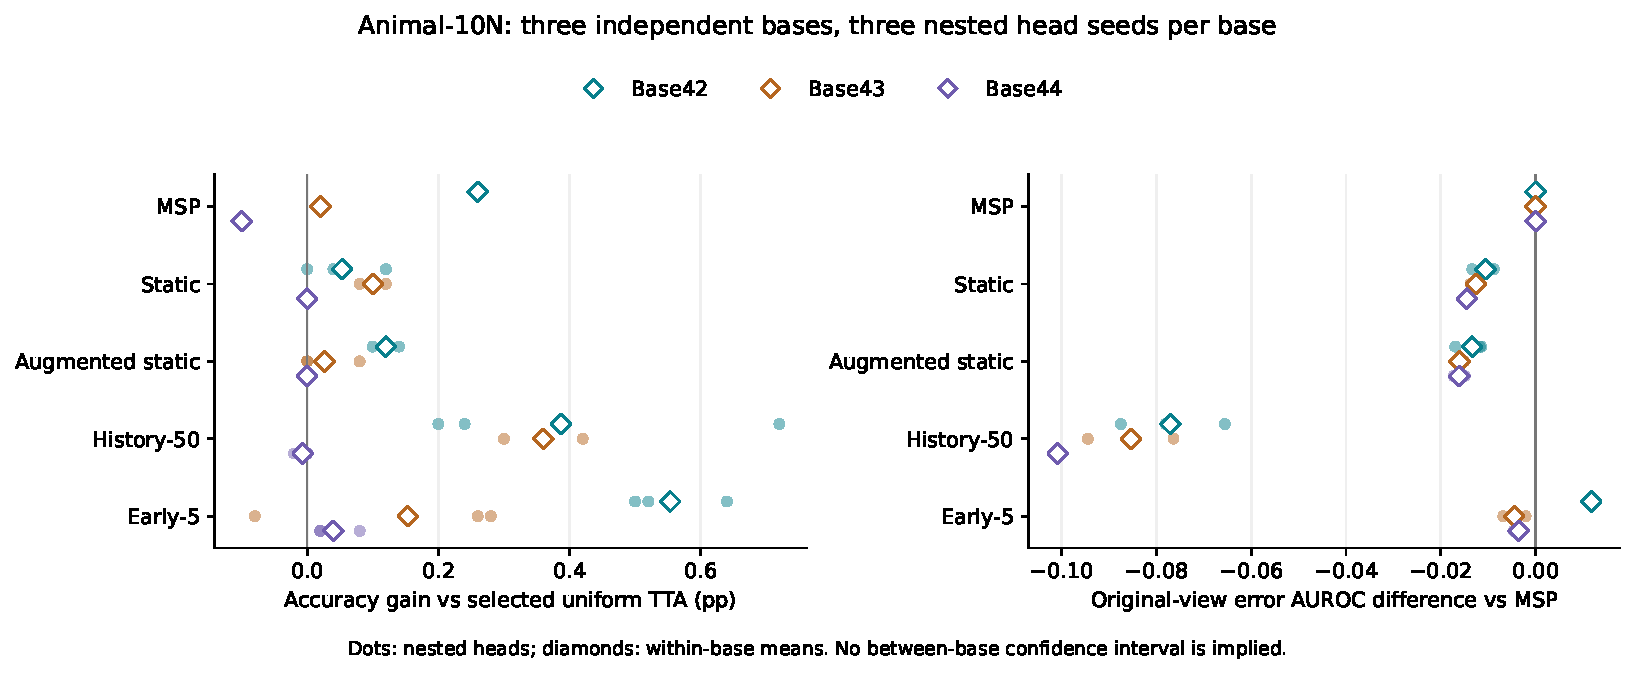
\includegraphics[width=\linewidth]{figures/animal10n_replications.pdf}
\caption{Animal-10N transfer across three independent base initializations. Dots show nested heads, diamonds within-base means and colors base seeds. Left: accuracy relative to each base's validation-selected uniform TTA. Right: error-ranking AUROC relative to original-view MSP. There is no implied confidence interval across independent bases.}
\end{figure}

\section{Mini-WebVision transfer across three bases}
\label{sec:minipilot}
The fixed recipe was transferred to the first 50 original classes of WebVision1.0,
using 65,944 Google training images and 2,500 official validation images for final
evaluation. A fixed noisy split reserves 6,594 training images for checkpoint and
policy selection; the remaining 59,350 supply training trajectories. Three
independent base initializations 42/43/44 each use three nested head seeds.
All 50 epochs completed; noisy-validation CE selected epochs 2/3/3 respectively.
The dataset realization, split and scientific configuration agree across bases.

All bases required recovery after memory-related interruption: base 42 resumed
after 40 epochs, with loader workers reduced from 4 to 0; bases 43/44 used workers 0
throughout and resumed after 43 epochs. Saved optimizer, RNG and target/history
state were restored. The corresponding history prefixes match exactly; a
bit-identical counterfactual uninterrupted run is not asserted.

\begin{table}[t]
\centering
\begin{tabular}{lrrrrr}
\toprule
Method & Base42 & Base43 & Base44 & Mean & Error AUROC \\
\midrule
FP32 base & 83.48 & 82.92 & 82.32 & 82.91 & 0.8853 \\
Uniform TTA & 83.24 & 83.32 & 83.44 & 83.33 & 0.8853 \\
Static & 83.32 & 83.47 & 83.48 & 83.42 & 0.8662 \\
Augmented static & 83.27 & 83.41 & 83.49 & 83.39 & 0.8645 \\
History-50 & 83.65 & 83.92 & 83.79 & 83.79 & 0.7541 \\
Early-5 & 84.13 & 83.83 & 84.29 & 84.08 & 0.8897 \\
\bottomrule
\end{tabular}

\caption{Mini-WebVision accuracy (\%) across independent bases. Learned methods
average three nested heads per base, then bases equally. They are not ensembles.
Error AUROC is the equally weighted mean for original-view FP32 base errors.
Each method uses its own noisy-validation policy.}
\label{tab:minipilot}
\end{table}

Early-5 accuracies are 84.13/83.83/84.29\%, compared with selected uniform
TTA 83.24/83.32/83.44\% and augmented-static 83.27/83.41/83.49\%.
Mean gains over TTA and the augmentation control are 0.75 and 0.69 percentage
points, positive on every base. The between-base sample SD of gains over TTA
is 0.21 points, not a confidence interval. Only three of nine nominal conditional
per-head accuracy intervals strictly exclude zero for each comparison; three
touch zero against TTA and two touch zero against the augmentation control.
These nine heads span only three independent bases and share the evaluation set.

History-50 obtains 83.65/83.92/83.79\% accuracy. Early-5 gains 0.48/-0.09/0.51 points,
averaging 0.30 points; only two of nine conditional accuracy intervals are strictly
positive. Early-5 therefore does not dominate full-history averaging on every
base. Mean original-view error AUROC is 0.8897 versus MSP 0.8853 and History-50
0.7541; the Early-5 mean exceeds MSP on each base, but no paired significance
claim against MSP follows from these point estimates. All nine nominal paired
AUROC intervals against History-50 and augmented-static are positive.

Mean Early-5 ECE/NLL are 0.0195/0.5803, compared with TTA 0.0205/0.5849.
NLL improves over selected TTA on all three bases; ECE worsens on bases 43/44
despite its lower three-base mean. History-50 has lower mean ECE (0.0171).
Accuracy, error ranking and calibration therefore require separate interpretation.

\begin{figure}[t]
\centering
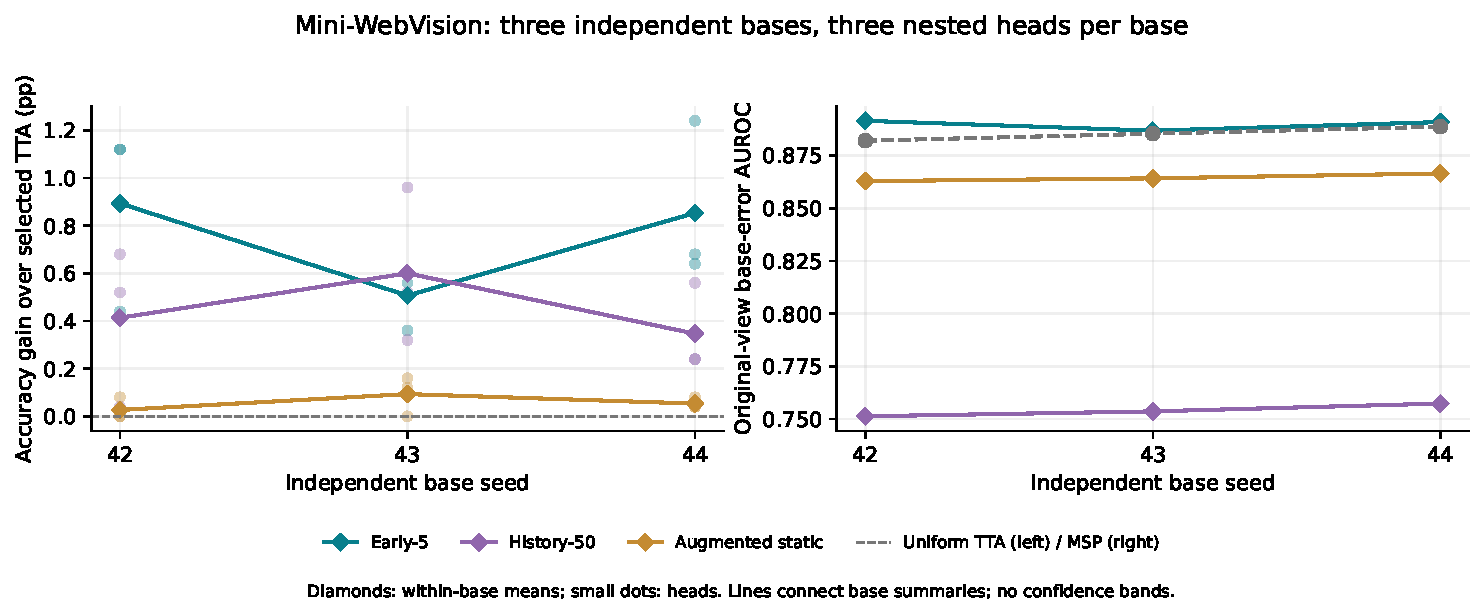
\includegraphics[width=\linewidth]{figures/miniwebvision_replications.pdf}
\caption{Mini-WebVision: within-base means across three independent initializations.
Small dots show nested head gains; connecting lines are not confidence bands.}
\label{fig:minipilot}
\end{figure}

The resumed pipelines took 2.32/2.04/1.96 hours, excluding image preparation and
all earlier interrupted work. Training-stage AMP base accuracies are
83.44/82.88/82.32\%; downstream comparisons consistently use the separately
recorded FP32 values83.48/82.92/82.32\%. Saved compact tables, policy choices
and checkpoint digests agree, but raw-prediction replay remains unperformed.
ImageNet pretraining overlaps the benchmark category space, so this is neither
unseen-category transfer nor a directly comparable state-of-the-art claim.

\section{Limitations}
\paragraph{Replication and adaptive development.}
The CIFAR evidence covers one base architecture with ImageNet initialization, two human-noise datasets, and six completed base runs (three per dataset). Section~\ref{sec:animalpilot} adds three prospectively planned Animal-10N base initializations with three nested heads per base. The transfer ties History-50 in mean accuracy and worsens error-ranking AUROC against MSP on two bases, limiting dataset-general claims. Head-seed standard deviations are not estimates of base-training variance. Repeated test inspection and the exploratory window study limit confirmatory interpretation of the nominal intervals. Section~\ref{sec:minipilot} adds three Mini-WebVision bases with positive gains over TTA and augmented static, but only three of nine conditional accuracy intervals strictly exclude zero for each comparison. Additional noise conditions and clean-training controls remain untested; raw-prediction replay on Mini-WebVision is pending.

\paragraph{Mechanism and supervision shift.}
The first-five-epoch target overlaps the cross-entropy warmup, and selected base checkpoints come from epochs 2 or 3, inside that warmup. The experiments do not separate early-learning information from the loss transition or checkpoint timing. Regression sees observed classes on base-training images; inference conditions on predicted classes of new views. The resulting score is useful empirically but has no calibration guarantee as a probability of error or annotation corruption. Full-history averaging also discards temporal order, so its comparison with Early-5 does not test every way of representing a complete trajectory.

\paragraph{Baselines and cost.}
The two-base ensemble has higher CIFAR-100N accuracy, and its two forward passes cannot be equated with our five or ten views. Direct learned view aggregation, alternative robust-training recipes, ensemble timing, and independent runtime replications remain necessary to establish the breadth and computational value of the approach. Calibration also remains a separate issue: better error ranking and accuracy coexist with worse CIFAR-100N ECE and NLL, and CIFAR-10N ECE changes direction across bases. The weakest new CIFAR-100N head has a nominal interval including zero relative to its base. The augmentation control now covers all six bases, including a rebuilt study on the verified original CIFAR-10N base42 checkpoint. Seven of nine CIFAR-100N head-level accuracy intervals are positive; the remaining two include zero on base44. All nine CIFAR-10N intervals are positive. These are three independent bases per dataset, not nine base replications. Fixed-checkpoint augmentation does not match the evolving training weights. The single-session T4 microbenchmark uses only four fixed validation images and is preliminary; small observed timing differences have no interval across independent timing runs.


\paragraph{Posterior-compression controls.}
The separate S2 posterior branch does not establish a distinct residual-head
advantage: Early-5 residual accuracy averages71.61\%, versus71.53\% for a direct
soft-target head and71.55\% for Early-2. Independent teachers produce71.87\% but
require additional base training and share donors across recipient comparisons.
These controls reuse a known test. Local raw-prediction replay cannot regenerate
fitting without the weights and train/validation arrays omitted from small
exports. The original seed42 full epoch-selection grid was subsequently recovered
and its ranking verified against the frozen policy.
The supplementary tie-aware AURC is explicitly separate from historical risk-area
calculations. The S2 and S4 T4 benchmarks measure inference latency under fixed batch and preprocessing settings. Training cost remains unmatched across teacher constructions.

\paragraph{Scope of the CIFAR-10.2 contrast.}
The matched comparison varies the source of teacher diversity, with five
early checkpoints on canonical images or five views from one early
checkpoint. It does not isolate the order of training states or quantify
variation over architectures and training recipes. The secondary
teacher comparison measures performance with five passes.

\section{Conclusion}
Room for Doubt transfers an early training-margin summary to inference through class-conditioned regression on frozen base features. Matched scalar controls show higher accuracy for Early-5 than for the selected checkpoint margin or the mean of all 50 epochs in the CIFAR runs. The gain appears on three independently trained CIFAR-100N bases and on three CIFAR-10N Worse bases, alongside improved ranking of original-view base errors. The augmentation control retains an Early-5 advantage on all three CIFAR-100N bases and all three CIFAR-10N bases, with positive conditional accuracy intervals for seven of nine CIFAR-100N heads and all nine CIFAR-10N heads. Preliminary T4 timing is close to equal-view uniform TTA, while multiple views remain costly. Calibration, causal interpretation and comparison with multi-model inference require further study.

The frozen Animal-10N transfer across three independent bases yields a smaller mean 0.25-point gain over uniform TTA. Early-5 and History-50 have virtually identical mean accuracy; most accuracy intervals against the augmentation-matched control include zero, and original-view AUROC falls below MSP on two bases. Thus transfer is feasible but the relative benefit depends on the dataset and base initialization; the evidence does not establish a universal advantage for the early summary.

Three Mini-WebVision bases retain positive Early-5 gains over selected TTA and the augmentation-matched static control, averaging 0.75 and 0.69 points. History-50 slightly exceeds Early-5 on one base, and only three of nine conditional accuracy intervals exclude zero for each comparison against TTA and augmented static. These replications broaden transfer evidence while retaining uncertainty about small accuracy gains and calibration.


A separate posterior-compression branch improves mean accuracy from
69.60\% to 71.61\% on the exploratory CIFAR-100N benchmark at near-base
latency. In a prespecified evaluation on CIFAR-10.1 v6, the same residual
recipe gives a mean change of $-0.07$ percentage points versus its base
(conditional paired 95\% interval $[-0.53, 0.42]$) and meets the latency
criterion. Direct distillation gains 0.57 points in a secondary comparison.

On CIFAR-10.2, the five-checkpoint teacher exceeds a five-view static
teacher by 2.10 percentage points in a secondary comparison. After
direct distillation, the prespecified contrast is $-0.02$ points
(conditional paired 95\% interval $[-0.53, 0.48]$).

\bibliography{references}
\bibliographystyle{icomp2026_conference}
\clearpage
\appendix
\section{Per-head Paired Intervals}
\label{app:intervals}
Table~\ref{tab:intervals} reports nominal 95\% paired test-example intervals for the primary Early-5 base-feature estimator. Gains and bounds are percentage points. The TTA reference in each interval uses the same view count as that head, which can differ from the globally validation-selected uniform-TTA policy in Table~\ref{tab:accuracy}. No interval here compares independently sampled datasets or directly tests Early-5 against the static regressor.
\begin{table}[!ht]
\centering\scriptsize
\caption{Primary estimator: saved validation-selected policies and conditional paired intervals.}
\label{tab:intervals}
\begin{tabular}{llrrrrr}
\toprule
Run & Head seed & Views & $T$ & Gain & CI vs base & CI vs same-view TTA \\
\midrule
C100, base 42 & 42 & 5 & 0.05 & +1.10 & [+0.57, +1.65] & [+0.61, +1.49] \\
C100, base 42 & 43 & 5 & 0.02 & +1.10 & [+0.54, +1.63] & [+0.56, +1.53] \\
C100, base 42 & 44 & 5 & 0.05 & +0.68 & [+0.15, +1.24] & [+0.20, +1.07] \\
C100, base 43 & 42 & 5 & 0.05 & +1.20 & [+0.70, +1.73] & [+0.86, +1.68] \\
C100, base 43 & 43 & 5 & 0.02 & +0.97 & [+0.42, +1.53] & [+0.58, +1.51] \\
C100, base 43 & 44 & 5 & 0.05 & +0.98 & [+0.48, +1.52] & [+0.63, +1.50] \\
C10 Worse, base 42 & 42 & 10 & 0.02 & +1.31 & [+0.88, +1.76] & [+0.50, +1.22] \\
C10 Worse, base 42 & 43 & 10 & 0.02 & +1.34 & [+0.90, +1.79] & [+0.52, +1.26] \\
C10 Worse, base 42 & 44 & 10 & 0.02 & +1.32 & [+0.87, +1.79] & [+0.51, +1.24] \\
\bottomrule
\end{tabular}

\end{table}

\clearpage
\section{Calibration and Error Ranking}
\label{app:calibration}
AUROC uses original-view scores and fixed original-view base-error labels. ECE, NLL, and Brier use the final probabilities of each method's selected policy. Therefore the ranking and calibration columns refer to explicitly different evaluation objects. Figure~\ref{fig:calibration_changes} shows changes relative to the corresponding base. All values for learned heads are arithmetic means over three head seeds; no seed is chosen by test performance.
\begin{table}[!ht]
\centering\scriptsize
\caption{Error AUROC and final-probability calibration. Lower ECE, NLL, and Brier are better.}
\label{tab:calibration}
\begin{tabular}{llrrrr}
\toprule
Run & Method & AUROC $\uparrow$ & ECE $\downarrow$ & NLL $\downarrow$ & Brier $\downarrow$ \\
\midrule
C100, base 42 & Base & 0.8124 & 0.1200 & 1.1253 & 0.4362 \\
C100, base 42 & Uniform TTA & 0.8124 & 0.1610 & 1.1670 & 0.4500 \\
C100, base 42 & Entropy weighting & 0.7647 & 0.1610 & 1.1670 & 0.4500 \\
C100, base 42 & Static & 0.8045 & 0.1554 & 1.1587 & 0.4465 \\
C100, base 42 & History-50 & 0.7112 & 0.1459 & 1.1570 & 0.4434 \\
C100, base 42 & Early-5 & 0.8307 & 0.1291 & 1.1404 & 0.4348 \\
C100, base 43 & Base & 0.8222 & 0.0963 & 1.1313 & 0.4358 \\
C100, base 43 & Uniform TTA & 0.8222 & 0.1436 & 1.1814 & 0.4503 \\
C100, base 43 & Entropy weighting & 0.7799 & 0.1436 & 1.1814 & 0.4503 \\
C100, base 43 & Static & 0.7984 & 0.1433 & 1.1810 & 0.4501 \\
C100, base 43 & History-50 & 0.6953 & 0.1335 & 1.1707 & 0.4434 \\
C100, base 43 & Early-5 & 0.8326 & 0.1098 & 1.1541 & 0.4363 \\
C100, base 44 & Base & 0.8281 & 0.0888 & 1.1082 & 0.4286 \\
C100, base 44 & Uniform TTA & 0.8281 & 0.0888 & 1.1082 & 0.4286 \\
C100, base 44 & Entropy weighting & 0.7874 & 0.0888 & 1.1082 & 0.4286 \\
C100, base 44 & Static & 0.8059 & 0.0888 & 1.1082 & 0.4286 \\
C100, base 44 & History-50 & 0.7097 & 0.1124 & 1.1476 & 0.4402 \\
C100, base 44 & Early-5 & 0.8325 & 0.0989 & 1.1375 & 0.4338 \\
C10 Worse, base 42 & Base & 0.8764 & 0.2847 & 0.6203 & 0.2677 \\
C10 Worse, base 42 & Uniform TTA & 0.8764 & 0.3155 & 0.6532 & 0.2841 \\
C10 Worse, base 42 & Entropy weighting & 0.8048 & 0.2464 & 0.5601 & 0.2373 \\
C10 Worse, base 42 & Static & 0.8853 & 0.3033 & 0.6382 & 0.2757 \\
C10 Worse, base 42 & History-50 & 0.7689 & 0.2888 & 0.6260 & 0.2687 \\
C10 Worse, base 42 & Early-5 & 0.9064 & 0.2756 & 0.5903 & 0.2481 \\
C10 Worse, base 43 & Base & 0.8758 & 0.2518 & 0.5591 & 0.2420 \\
C10 Worse, base 43 & Uniform TTA & 0.8758 & 0.2893 & 0.5903 & 0.2559 \\
C10 Worse, base 43 & Entropy weighting & 0.8312 & 0.2877 & 0.5877 & 0.2546 \\
C10 Worse, base 43 & Static & 0.8792 & 0.2886 & 0.5890 & 0.2552 \\
C10 Worse, base 43 & History-50 & 0.7398 & 0.2673 & 0.5659 & 0.2422 \\
C10 Worse, base 43 & Early-5 & 0.8976 & 0.2542 & 0.5359 & 0.2254 \\
C10 Worse, base 44 & Base & 0.8571 & 0.2638 & 0.6009 & 0.2630 \\
C10 Worse, base 44 & Uniform TTA & 0.8571 & 0.2907 & 0.6304 & 0.2768 \\
C10 Worse, base 44 & Entropy weighting & 0.7994 & 0.2907 & 0.6304 & 0.2768 \\
C10 Worse, base 44 & Static & 0.8693 & 0.2566 & 0.5913 & 0.2551 \\
C10 Worse, base 44 & History-50 & 0.7687 & 0.2764 & 0.6086 & 0.2639 \\
C10 Worse, base 44 & Early-5 & 0.9156 & 0.2672 & 0.5781 & 0.2466 \\
\bottomrule
\end{tabular}

\end{table}

\begin{figure}[!ht]
\centering
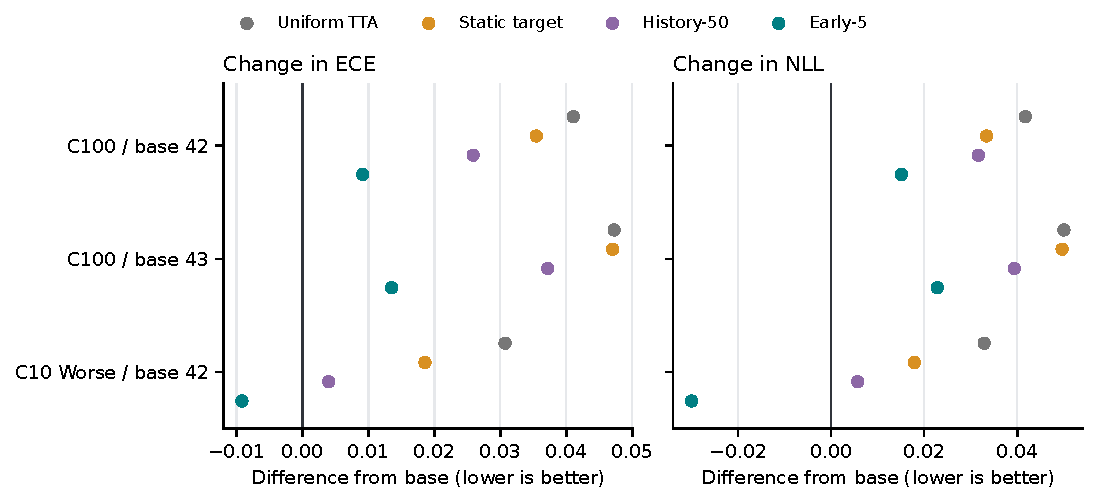
\includegraphics[width=\linewidth]{figures/calibration_changes.pdf}
\caption{Change in final-probability calibration relative to the corresponding base. Points average learned heads where applicable. Positive values mean worse ECE or NLL. These are point estimates, not confidence intervals; methods use their own validation-selected policies.}
\label{fig:calibration_changes}
\end{figure}

\clearpage
\section{Reconstruction of the Regression Targets}
Table~\ref{tab:reconstruction} measures prediction of the corresponding scalar target on the 6,750 diagnostic IDs excluded from PCA fitting, head fitting, and head checkpoint selection. These images were seen by the base during its training. The static target has higher $R^2$ than Early-5 on every base despite lower downstream accuracy. Absolute MSE values refer to different target distributions and should not be read as a common-scale ranking of usefulness. Values are averaged over three head seeds, separately for each base.
\begin{table}[!ht]
\centering\small
\caption{Diagnostic-held-out target reconstruction using base features. $R^2$ is relative to each target's own variance; it is not error-detection AUROC.}
\label{tab:reconstruction}
\begin{tabular}{llrr}
\toprule
Run & Target & MSE & $R^2$ \\
\midrule
C100, base 42 & Early-5 & 0.0519 & 0.754 \\
C100, base 42 & Static & 0.0493 & 0.838 \\
C100, base 42 & History-50 & 0.1085 & 0.524 \\
C100, base 43 & Early-5 & 0.0511 & 0.753 \\
C100, base 43 & Static & 0.0542 & 0.828 \\
C100, base 43 & History-50 & 0.1066 & 0.539 \\
C100, base 44 & Early-5 & 0.0538 & 0.743 \\
C100, base 44 & Static & 0.0589 & 0.816 \\
C100, base 44 & History-50 & 0.1087 & 0.547 \\
C10 Worse, base 42 & Early-5 & 0.0187 & 0.917 \\
C10 Worse, base 42 & Static & 0.0051 & 0.980 \\
C10 Worse, base 42 & History-50 & 0.0748 & 0.810 \\
C10 Worse, base 43 & Early-5 & 0.0182 & 0.918 \\
C10 Worse, base 43 & Static & 0.0055 & 0.982 \\
C10 Worse, base 43 & History-50 & 0.0759 & 0.808 \\
C10 Worse, base 44 & Early-5 & 0.0178 & 0.921 \\
C10 Worse, base 44 & Static & 0.0050 & 0.982 \\
C10 Worse, base 44 & History-50 & 0.0740 & 0.812 \\
\bottomrule
\end{tabular}

\end{table}

\section{Reproducibility Details}
The regressor's scalar output is internally broadcast to 50 entries for compatibility with the existing trajectory-prediction interface. MSE over this repeated target is mathematically the same scalar regression objective; it does not train 50 independent outputs. Stable sample IDs link trajectories, features, annotations, and views. PCA is fitted separately for each encoder using only meta-training features. The ResNet18 condition retains all 512 dimensions without whitening; the base-feature condition reduces 2048 dimensions to 512.

The observed-label static target uses an unaugmented forward pass at the selected checkpoint, while temporal targets use training-time augmentations and changing weights. The matched comparison holds the head and decision procedure fixed, but target construction differs in both temporal information and measurement conditions. A fixed-checkpoint target averaged over the same augmentation process would further separate those contributions.


\clearpage
\section{Follow-up Target Controls}
\label{app:followup_controls}
The follow-up covers CIFAR-100N base seed 44 and CIFAR-10N Worse base seed 43. It reuses frozen base features, the original train-only PCA, and the nine existing base-feature heads per base. Three new heads per base predict the mean observed-label margin over five augmentations at the minimum-noisy-validation-loss checkpoint. The transform is the actual base-training sequence: constant-padding random crop at $32\times32$, random horizontal flip, then ImageNet resize/normalization. This differs from the reflected-padding inference-view stream. Original training RNG draws were not recorded; the control samples new deterministic draws (seed 20261019). It neither matches online weight evolution nor separates the cross-entropy warmup from later GCE training.

All old validation-selected policies and downstream accuracy values reproduce. New policies freeze before test evaluation; clean training labels do not construct targets or fit heads. The two augmentation-control jobs together fit six new heads; no base is retrained. The complete follow-up batch, including direct comparisons and runtime measurements, takes 41.89 minutes. This is not the cost of one deployment head.

\begin{table}[!ht]
\centering\small
\caption{Follow-up accuracy (\%); mean $\pm$ sample SD over three heads on each base. Each method retains its own noisy-validation-selected policy.}
\label{tab:followup_accuracy}
\begin{tabular}{lrrr}
\toprule
Target & Base 42 & Base 43 & Base 44 \\
\midrule
\multicolumn{4}{l}{\textbf{CIFAR-100N}} \\
Static & 70.35 $\pm$ 0.10 & 69.27 $\pm$ 0.01 & 69.57 $\pm$ 0.00 \\
Aug-static & 70.32 $\pm$ 0.04 & 69.27 $\pm$ 0.02 & 69.57 $\pm$ 0.00 \\
History-50 & 70.46 $\pm$ 0.18 & 69.93 $\pm$ 0.09 & 69.68 $\pm$ 0.18 \\
Early-5 & 71.08 $\pm$ 0.24 & 70.28 $\pm$ 0.13 & 70.09 $\pm$ 0.21 \\
\multicolumn{4}{l}{\textbf{CIFAR-10N Worse}} \\
Static & 89.19 $\pm$ 0.13 & 90.53 $\pm$ 0.02 & 88.82 $\pm$ 0.10 \\
Aug-static & 89.28 $\pm$ 0.08 & 90.61 $\pm$ 0.05 & 88.91 $\pm$ 0.07 \\
History-50 & 89.01 $\pm$ 0.31 & 90.43 $\pm$ 0.12 & 89.35 $\pm$ 0.19 \\
Early-5 & 90.16 $\pm$ 0.02 & 91.28 $\pm$ 0.02 & 90.39 $\pm$ 0.15 \\
\bottomrule
\end{tabular}

\end{table}

Table~\ref{tab:followup_pairs} gives direct Early-5 minus reference contrasts for the base-feature heads. Accuracy intervals use 2,000 paired test-example draws. AUROC differences compare original-view scores against the same original-view base-error events; their intervals use 2,000 paired stratified draws retaining the observed error/correct counts, with bootstrap seed 20261019. They are nominal, conditional, exploratory intervals without multiplicity correction, not intervals over independently trained bases.

For Early-5 versus augmented-static, CIFAR-100N head-42/43/44 AUROC differences are 0.0259, 0.0260 and 0.0320, with intervals $[0.0198,0.0325]$, $[0.0195,0.0323]$, and $[0.0256,0.0383]$. CIFAR-10N differences are 0.0183, 0.0186 and 0.0168, with intervals $[0.0123,0.0239]$, $[0.0130,0.0238]$, and $[0.0107,0.0229]$. These positive ranking differences do not guarantee accuracy improvements or calibrated probabilities.

\begin{table}[!ht]
\centering\scriptsize
\caption{Direct paired target contrasts. Gain and CI are accuracy percentage points; $\Delta$AUROC refers to original-view error ranking. $V_r/V_e$ lists reference/Early-5 selected views.}
\label{tab:followup_pairs}
\begin{tabular}{lllrrrr}
\toprule
Run & Seed & Reference & $V_r/V_e$ & Gain & 95\% CI & $\Delta$AUROC \\
\midrule
C100/44 & 42 & Static & 1/5 & +0.53 & [+0.00, +1.04] & +0.0214 \\
C100/44 & 42 & History-50 & 5/5 & +0.42 & [+0.03, +0.79] & +0.1213 \\
C100/44 & 42 & Aug-static & 1/5 & +0.53 & [+0.00, +1.04] & +0.0259 \\
C100/44 & 43 & Static & 1/5 & +0.31 & [-0.20, +0.79] & +0.0248 \\
C100/44 & 43 & History-50 & 5/5 & +0.38 & [+0.01, +0.75] & +0.1151 \\
C100/44 & 43 & Aug-static & 1/5 & +0.31 & [-0.20, +0.79] & +0.0260 \\
C100/44 & 44 & Static & 1/10 & +0.72 & [+0.14, +1.29] & +0.0334 \\
C100/44 & 44 & History-50 & 5/10 & +0.44 & [-0.07, +0.93] & +0.1319 \\
C100/44 & 44 & Aug-static & 1/10 & +0.72 & [+0.14, +1.29] & +0.0320 \\
C10/43 & 42 & Static & 10/10 & +0.76 & [+0.47, +1.06] & +0.0147 \\
C10/43 & 42 & History-50 & 10/10 & +0.75 & [+0.46, +1.05] & +0.1748 \\
C10/43 & 42 & Aug-static & 10/10 & +0.67 & [+0.39, +0.96] & +0.0183 \\
C10/43 & 43 & Static & 10/5 & +0.74 & [+0.41, +1.08] & +0.0232 \\
C10/43 & 43 & History-50 & 5/5 & +1.00 & [+0.70, +1.33] & +0.1707 \\
C10/43 & 43 & Aug-static & 10/5 & +0.64 & [+0.32, +0.97] & +0.0186 \\
C10/43 & 44 & Static & 10/10 & +0.74 & [+0.41, +1.09] & +0.0172 \\
C10/43 & 44 & History-50 & 5/10 & +0.79 & [+0.45, +1.14] & +0.1278 \\
C10/43 & 44 & Aug-static & 5/10 & +0.70 & [+0.38, +1.04] & +0.0168 \\
\bottomrule
\end{tabular}

\end{table}

\begin{figure}[!ht]
\centering
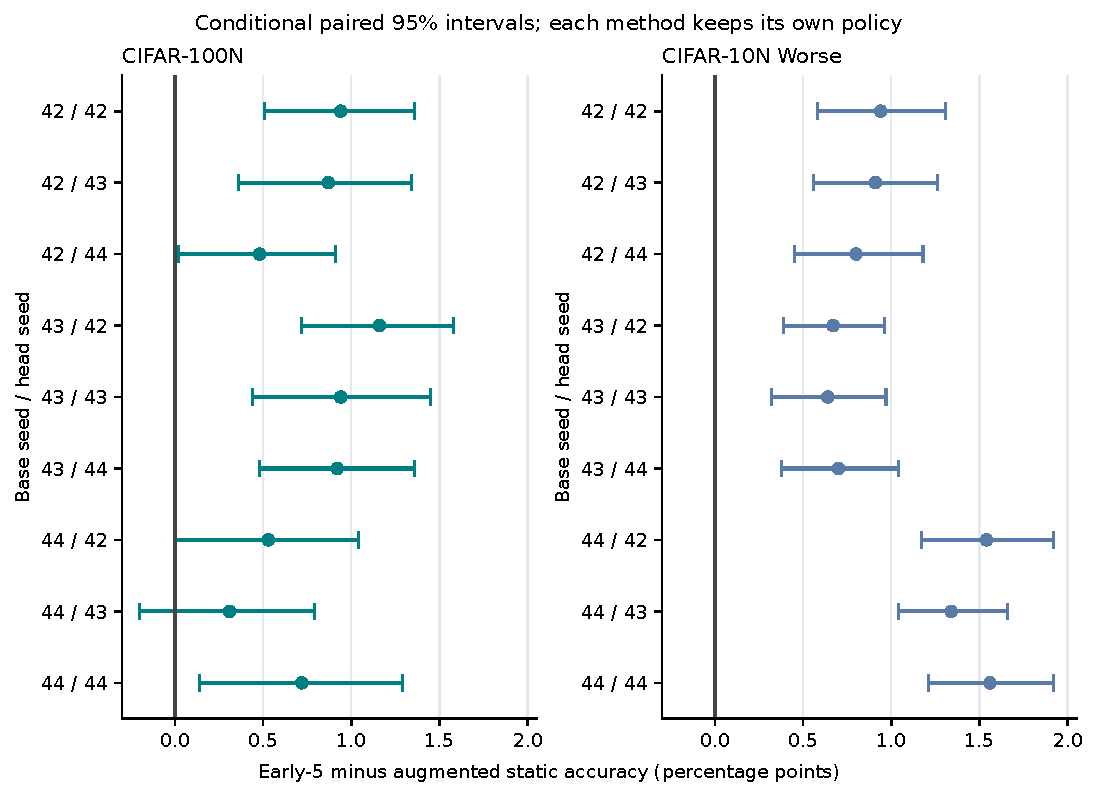
\includegraphics[width=\linewidth]{figures/augmentation_control.pdf}
\caption{Early-5 minus augmented-static accuracy. Bars are nominal 95\% paired test-example intervals conditional on each fitted base/head and selected policy, without multiplicity correction. They do not estimate base-training uncertainty. The policies can select different view counts.}
\label{fig:augmentation_control}
\end{figure}

\clearpage
\section{Matched Inference Microbenchmark}
\label{app:runtime}
A single Tesla T4 session runs sequentially on CIFAR-100N base44 and CIFAR-10N base43 using PyTorch 2.11.0+cu128, FP32 and four CPU threads. Head seed42 is fixed. Each timing configuration uses five warmups and 30 synchronized repetitions. Batch sizes 1/4 and view counts 1/5/10 are predefined; images are the first four fixed noisy-validation IDs, with shared deterministic view prefixes. Neither accuracy nor labels select timing cases. Temperatures come from each saved view budget's validation policy, rather than the globally selected view count. This reference inference path fuses the selected base features, PCA and the scalar head; cache generation and model/disk loading are outside the timing scope.

Table~\ref{tab:runtime} reports batch-size-one medians. The model scope starts from device tensors; the preprocessing scope includes CPU view generation, normalization and host-to-device transfer. Full CSVs retain batch medians/p95, batch-four amortized cost and GPU allocation measurements. Batch-four p95 is not per-image p95. Peak MB means PyTorch-allocated CUDA memory in decimal MB, not total device memory. Uniform/single-view policies skip the head.

\begin{table}[!ht]
\centering\small
\caption{Single-image inference medians (ms), head42 on one T4. Peak MB is allocated memory for the preprocessing-inclusive scope. Comparisons use the same view budget; these are not independent timing replications.}
\label{tab:runtime}
\begin{tabular}{llrrrr}
\toprule
Run & Method & Views & Model ms & With prep. ms & Peak MB \\
\midrule
C100/44 & Base & 1 & 7.68 & 7.59 & 133.9 \\
C100/44 & Uniform & 5 & 15.86 & 20.25 & 161.4 \\
C100/44 & Early-5 & 5 & 15.89 & 20.36 & 166.3 \\
C100/44 & Uniform & 10 & 30.42 & 40.05 & 215.1 \\
C100/44 & Early-5 & 10 & 30.46 & 40.40 & 219.8 \\
C10/43 & Base & 1 & 6.51 & 7.52 & 133.2 \\
C10/43 & Uniform & 5 & 16.47 & 20.82 & 160.7 \\
C10/43 & Early-5 & 5 & 16.66 & 20.46 & 165.5 \\
C10/43 & Uniform & 10 & 31.80 & 40.93 & 214.3 \\
C10/43 & Early-5 & 10 & 31.94 & 41.01 & 219.1 \\
\bottomrule
\end{tabular}

\end{table}

At five/ten views the observed extra allocated peak memory is about 4.8 MB for the PCA/head. Multi-view prediction is substantially costlier than a one-view base pass. Close matched-view medians are preliminary: one session, a fixed measurement order, a tiny fixed image set, and no independent timing intervals preclude a precise overhead guarantee. Separate one-view cases using equivalent computations also exhibit timing variation. No two-base ensemble is timed. These results do not establish lower latency than an ensemble or the cost of separately returning a standalone error-ranking score for every image.

\section{Separate Temporal Compression Pilot}
\label{sec:temporal-residual-validation}

This appendix records a separate exploratory redesign, not an extension of the
scalar method's test results. One new CIFAR-100N base (initialization42, fixed
split 42) completed 50 epochs, retaining end-of-epoch snapshots 1--5 before a separate frozen
clean-test evaluation. These snapshots supplied full class probabilities on
identical canonical training images. A residual MLP on the selected base's frozen
2048-dimensional features was fitted to their mean by KL divergence. Its hidden
width is 256, its output layer starts at zero, and it uses the original reserved
meta partitions. The deployed posterior is
$\operatorname{softmax}(\log p_{\mathrm{base}}+\alpha h(f(x)))$.
The head checkpoint minimizes reserved meta-validation KL; the fixed
$\alpha\in\{0,.25,.5,1\}$ grid uses noisy base-validation accuracy, then cross
entropy, then smaller $\alpha$. No policy was selected on clean test data.

\begin{table}[h]
\centering
\caption{Single-base noisy-validation pilot (5,000 observed labels). These are
not clean-test accuracies or significance estimates.}
\begin{tabular}{lrrr}
\toprule
Predictor & Accuracy (\%) & Gain (pp) & NLL\\
\midrule
Selected base(FP32) &54.66&0.00&1.916\\
Residual student &56.08&1.42&1.861\\
Five-snapshot mean &56.56&1.90&1.826\\
\bottomrule
\end{tabular}
\end{table}

Both selected interpolation strengths are 1. The base checkpoint is epoch 2
(one-based), and the residual checkpoint is epoch 4 of 25. Meta-validation KL
falls from 0.1249 at initialization to 0.06872, while later training continues to
reduce fitting KL without improving the selected validation minimum. The ratio
$1.42/1.90\approx.747$ describes retained noisy-validation gain on this split;
it is not a cross-dataset transfer guarantee. Reuse of noisy validation for
checkpoint and strength selection limits interpretation. The compact export
supports 35 consistency checks but contains neither binary weights nor per-image
probabilities, so no paired interval or raw replay is claimed.

This mechanism compresses a snapshot mean and is related to existing snapshot
distillation; no new temporal-attribution or novelty claim is established here.
The following subsection records independent-base follow-ups; matched
non-temporal ensemble controls remain outstanding. The main manuscript's scalar results are unchanged.

\begin{figure}[ht]
\centering
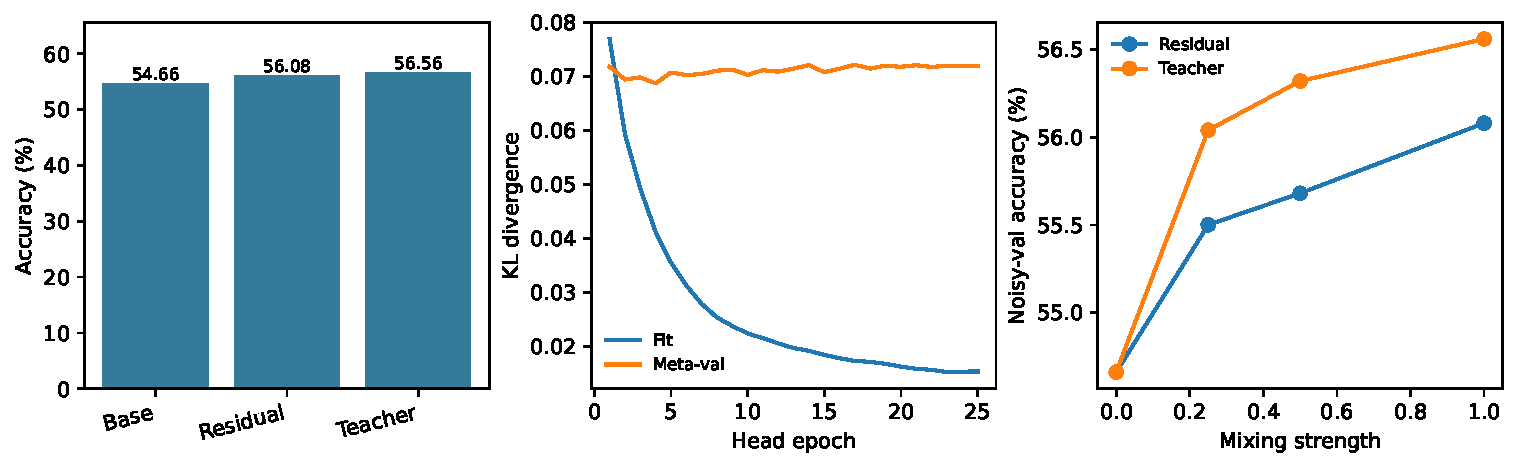
\includegraphics[width=\textwidth]{figures/temporal_residual_validation.pdf}
\caption{Validation-only pilot: selected accuracies, head fitting curves, and
the complete fixed strength grid. One base and one head initialization; no
test-result or significance interval is shown.}
\end{figure}

\subsection{Frozen Clean-Test Evaluation}

The already selected policy and checkpoint were evaluated without refitting or
changing either interpolation strength. Source, checkpoint, evidence-cache and
policy identities were checked before test access. Saved per-image probabilities
on all 10,000 official CIFAR-100 test images reproduce the exported metrics and
paired intervals; 46 local replay checks passed.

\begin{table}[ht]
\centering
\caption{Separate frozen pilot, one fitted base and head. ECE uses 15 bins.
The five-snapshot teacher requires five backbone passes; the student uses one
backbone pass plus its residual MLP.}
\begin{tabular}{lrrrr}
\toprule
Predictor & Accuracy (\%) & NLL & Brier & ECE\\
\midrule
Selected base &69.79&1.1273&.4373&.1226\\
Residual student &71.83&1.0867&.4198&.1498\\
Five-snapshot mean &73.15&1.0442&.4087&.1620\\
\bottomrule
\end{tabular}
\end{table}

Student minus base accuracy is $+2.04$ percentage points, with nominal paired
95\% bootstrap interval $[1.46,2.65]$. Teacher minus base is $+3.36$
$[2.70,4.04]$ points; student minus teacher is $-1.32$ $[-1.86,-0.77]$ points.
These 2,000-draw intervals condition on the fitted models and test examples;
they have no multiplicity adjustment and do not estimate between-base variation.
The student retains $2.04/3.36=60.7\%$ of the teacher's accuracy gain.
NLL and Brier improve, while ECE worsens; hence improved calibration is not
claimed. Student own-error AUROC is .8313 versus .8169 for the base, but these
scores target different error events. Against the fixed original-base error
event, student confidence gives AUROC .8355. These single-base results support
feasibility, not a demonstrated temporal-specific advantage or broad robustness.

\begin{figure}[ht]
\centering
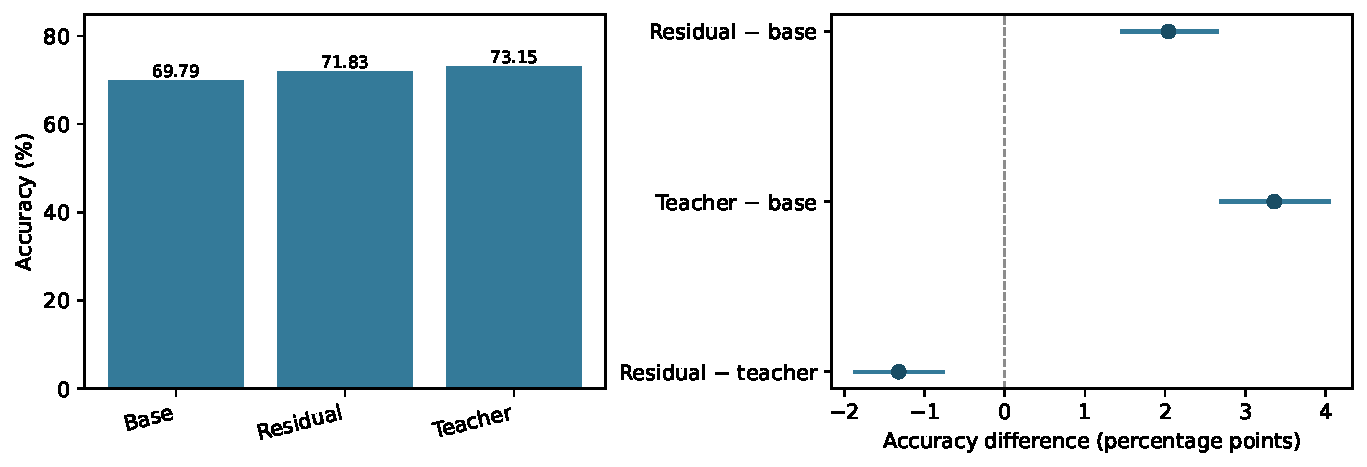
\includegraphics[width=\textwidth]{figures/temporal_residual_test.pdf}
\caption{Frozen clean-test accuracy and predeclared paired comparisons.
Intervals condition on one fitted base/head. No policy was selected on test.}
\end{figure}

\subsection{Independent-Base Follow-ups and Fixed Single-Epoch Control}

The follow-up protocol was specified after observing the seed42 pilot test,
not before that pilot. Independent base seeds43 and44 retain base split42,
the same 50-epoch training protocol and head seed42. Each base supports two
heads with identical features, meta partitions, initialization, optimizer,
25-epoch budget and validation selection: the mean of snapshots1--5, or the
single fixed epoch1 teacher. Both policies were frozen before either test was
accessed. Raw predictions reproduce all exported metrics and comparisons;
155 local checks passed. This control tests multiple-snapshot compression
against one fixed early snapshot, not an equal-compute independent ensemble.

\begin{table}[ht]
\centering
\caption{Clean-test accuracy (\%). Mean and sample SD describe three independent
base initializations with a fixed head seed and data split; SD is not a confidence
interval. The epoch1 control was run only for seeds43/44.}
\begin{tabular}{lrrrr}
\toprule
Base seed & Base & Temporal student & Five-snapshot mean & Epoch1 student\\
\midrule
42 &69.79&71.83&73.15&---\\
43 &69.98&71.45&73.55&71.13\\
44 &69.04&71.55&73.07&70.62\\
\midrule
Mean $\pm$ SD & $69.60\pm.50$ & $71.61\pm.20$ & $73.26\pm.26$ &---\\
\bottomrule
\end{tabular}
\end{table}

Student gains over the base are $+2.04$, $+1.47$ and $+2.51$ percentage points
(mean $+2.01$, sample SD $.52$). The later two conditional paired-example
intervals are $[1.06,1.88]$ and $[1.92,3.12]$ points. However, single-epoch
students also improve the base by $+1.15$ and $+1.58$ points. Temporal minus
single-epoch student is $+.32$ $[-.02,.68]$ points on seed43 and $+.93$
$[.43,1.45]$ points on seed44; the mean descriptive difference is $.625$ points.
The seed43 interval includes zero. These nominal intervals are unadjusted and
condition on the fitted models. Two control bases cannot establish robust
between-base superiority. ECE worsens relative to the base on all three seeds.
Thus compression gains replicate, but attributing all of the gain to temporal
history, or claiming improved calibration, is unsupported. Comparison against
stronger validation-selected single-snapshot and non-temporal ensemble controls
was pending at this stage; the S2 controls below address several of these gaps.
The strongest ensemble teacher still exceeds each student.

\begin{figure}[ht]
\centering
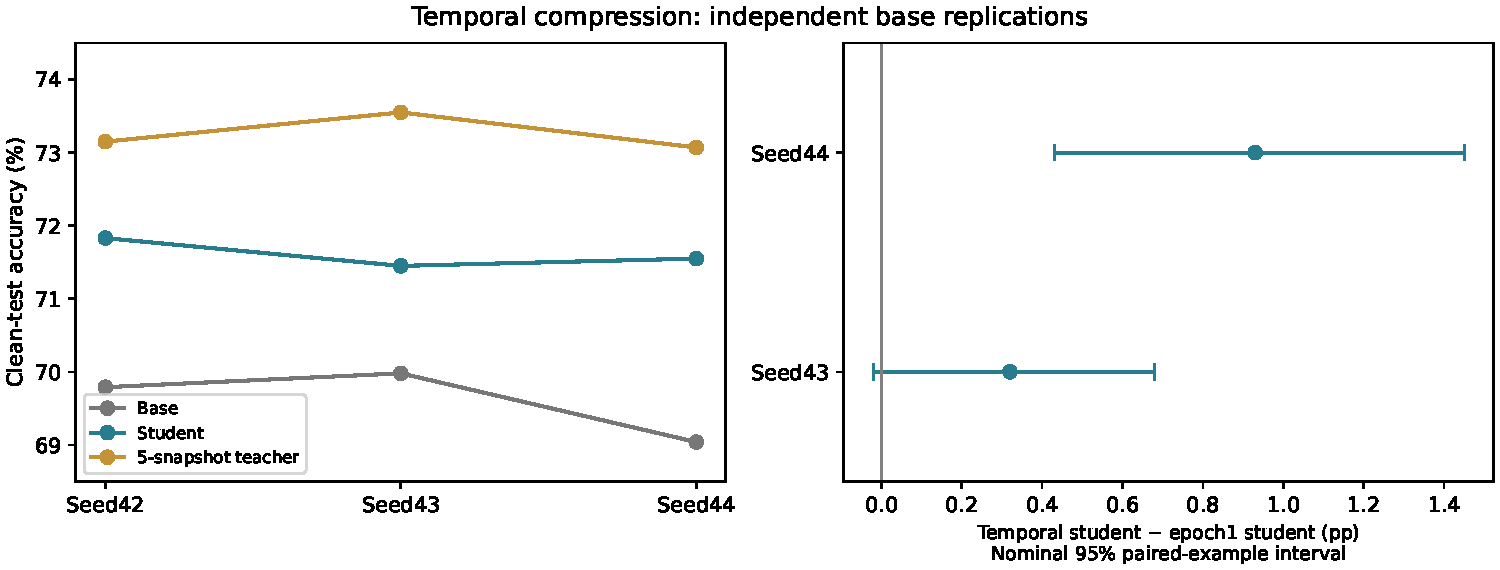
\includegraphics[width=\textwidth]{figures/temporal_residual_replications.pdf}
\caption{Independent base seeds and the fixed epoch1 head control.
Conditional intervals are not uncertainty across training runs.}
\end{figure}

\subsection{Exploratory Validation-Selected Single-Snapshot Control}

After the preceding test results were known, a stronger single-teacher control
was specified for base seeds43/44. Epochs1--5 and interpolation strengths
$\{0,.25,.5,1\}$ were ranked using noisy-validation accuracy, then lower NLL,
smaller strength and earlier epoch. The selected epochs are5 and3, respectively.
Identical residual heads and meta splits were used, with both control policies
frozen before their evaluation. Because the official test had already been
examined, this is explicitly post-pilot exploratory reuse, not independent
confirmatory evidence. Raw prediction replay passed81 checks.

\begin{table}[ht]
\centering
\caption{Validation-selected single-snapshot control. Accuracy in percent;
the two-pass interpolation uses the original base and selected teacher.}
\begin{tabular}{lrrrr}
\toprule
Seed & Base & Single student & Temporal student & Two-pass interpolation\\
\midrule
43&69.98&70.97&71.45&71.67\\
44&69.04&71.25&71.55&71.77\\
\bottomrule
\end{tabular}
\end{table}

Temporal minus selected-single student is $+.48$ points (nominal paired
95\% interval $[.10,.90]$) and $+.30$ points ($[-.17,.78]$). The descriptive
mean difference is $.39$ points across two bases, not a between-base significance
estimate. Substantial gains are therefore reproduced by single-snapshot
distillation, limiting attribution of the full base-relative improvement to
temporal aggregation. The simple two-pass interpolation is $.22$ points above
the temporal student on each base, although the conditional intervals for
this difference include zero. The latency of the one-pass student and the five-pass teacher was measured
separately on T4. The later CIFAR-10.1 evaluation did not confirm the
residual accuracy gain (Section~\ref{sec:confirmation-s4}).

\begin{figure}[ht]
\centering
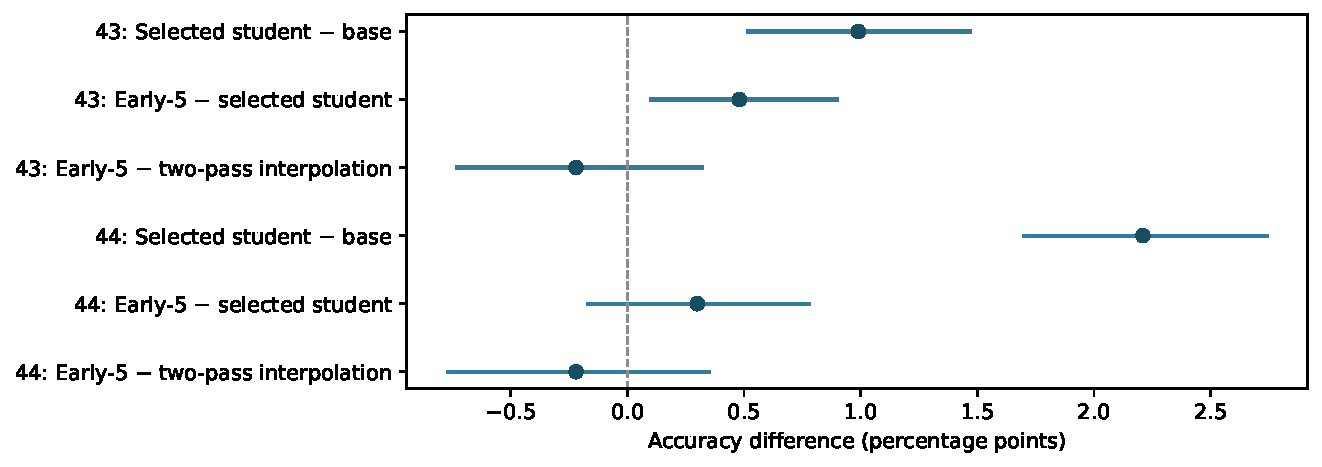
\includegraphics[width=\textwidth]{figures/temporal_selected_control.pdf}
\caption{Exploratory selected-single comparison. Two-pass interpolation is
reported separately from one-backbone-pass student heads.}
\end{figure}


\subsection{Exploratory S2 Post-Hoc Controls Across Three Bases}

Two frozen packages completed13 new heads:10 controls in A and three
independent-teacher students in B. The head seed remains42. All heads train on
noisy annotations or teacher probabilities; clean test labels are evaluation-only.
The direct soft-target head uses the same frozen features, Early-5 target and MLP
width as the residual head, without the base-log-probability offset during fitting;
both use validation-selected interpolation at inference. Early-2 averages states1
and5. Independent-2 averages the other two trained bases for each recipient.
Thus teacher pass counts match Early-2, but training costs do not: independent
teachers require additional base training and donors are shared between recipients.
The selected base checkpoint is epoch2 for all recipients, and states1--5 belong
to CE warmup. The contrasts cannot isolate a general causal effect of temporal
history from optimization phase or teacher quality.

\begin{table}[ht]
\centering
\caption{Exploratory CIFAR-100N controls: accuracy (\%). All student methods use one backbone pass. Means give equal weight to the three original bases; the head seed is fixed at42.}
\begin{tabular}{lrrrr}
\toprule
Method &42&43&44&Mean\\
\midrule
Base & 69.79 & 69.98 & 69.04 & 69.60\\
Selected single & 71.51 & 70.97 & 71.25 & 71.24\\
Noisy-label head & 71.13 & 71.45 & 70.84 & 71.14\\
Early-2 residual & 71.38 & 71.85 & 71.41 & 71.55\\
Early-5 residual & 71.83 & 71.45 & 71.55 & 71.61\\
Early-5 direct & 71.51 & 71.58 & 71.51 & 71.53\\
Independent-2 student & 71.95 & 71.81 & 71.84 & 71.87\\
\bottomrule
\end{tabular}
\end{table}


Early-5 exceeds the validation-selected single-snapshot student by .32, .48 and
.30 percentage points (mean .367). The nominal paired intervals include zero
for seeds42 and44. Its mean advantage over the direct soft-target head is only
.077 points; all three corresponding intervals include zero. Its mean advantage
over Early-2 is .063 points with mixed seed-wise signs. Independent-2 students
reach 71.87\% versus71.61\% for Early-5; shared donors and conditional intervals
preclude claiming independent, statistically established superiority. These
comparisons retain the base-relative compression gain while failing to establish
a distinctive benefit of the residual parametrization or five-state target.

Deterministic local replay of supplied raw predictions passed503 checks,
including source hashes, policy consistency, sample alignment, exported metrics
and paired comparisons. Cross-platform teacher interpolation matches within
$10^{-6}$ absolute and $2\times10^{-5}$ relative tolerance with exactly matching
class decisions; this is not bitwise reconstruction. Small exports omit fitted
weights and train/validation target arrays, so training and complete model-forward
regeneration were not performed locally. The seed42 full20-row epoch-selection
grid was subsequently recovered from original Kaggle Output version362957682.
Replaying its ranking exactly reproduces the frozen policy (epoch3, strength.5);
this closes the missing-grid gap without regenerating validation predictions.

Risk-coverage area was absent from the original S2 export. Supplemental local
analysis computes mean risk at discrete coverages with expected random ordering
inside exact confidence ties. Mean AURC is .11786 for the base, .10240 for Early-5,
.10394 for the direct head and .10197 for Independent-2. This tie-safe definition
is separate from historical risk-area exports. ECE remains worse for Early-5
than the base. GPU latency and end-to-end cost have not been measured; the
accuracy block does not complete the full S2 decision gate. All comparisons
reuse a previously examined test set and are exploratory.

\begin{figure}[ht]
\centering
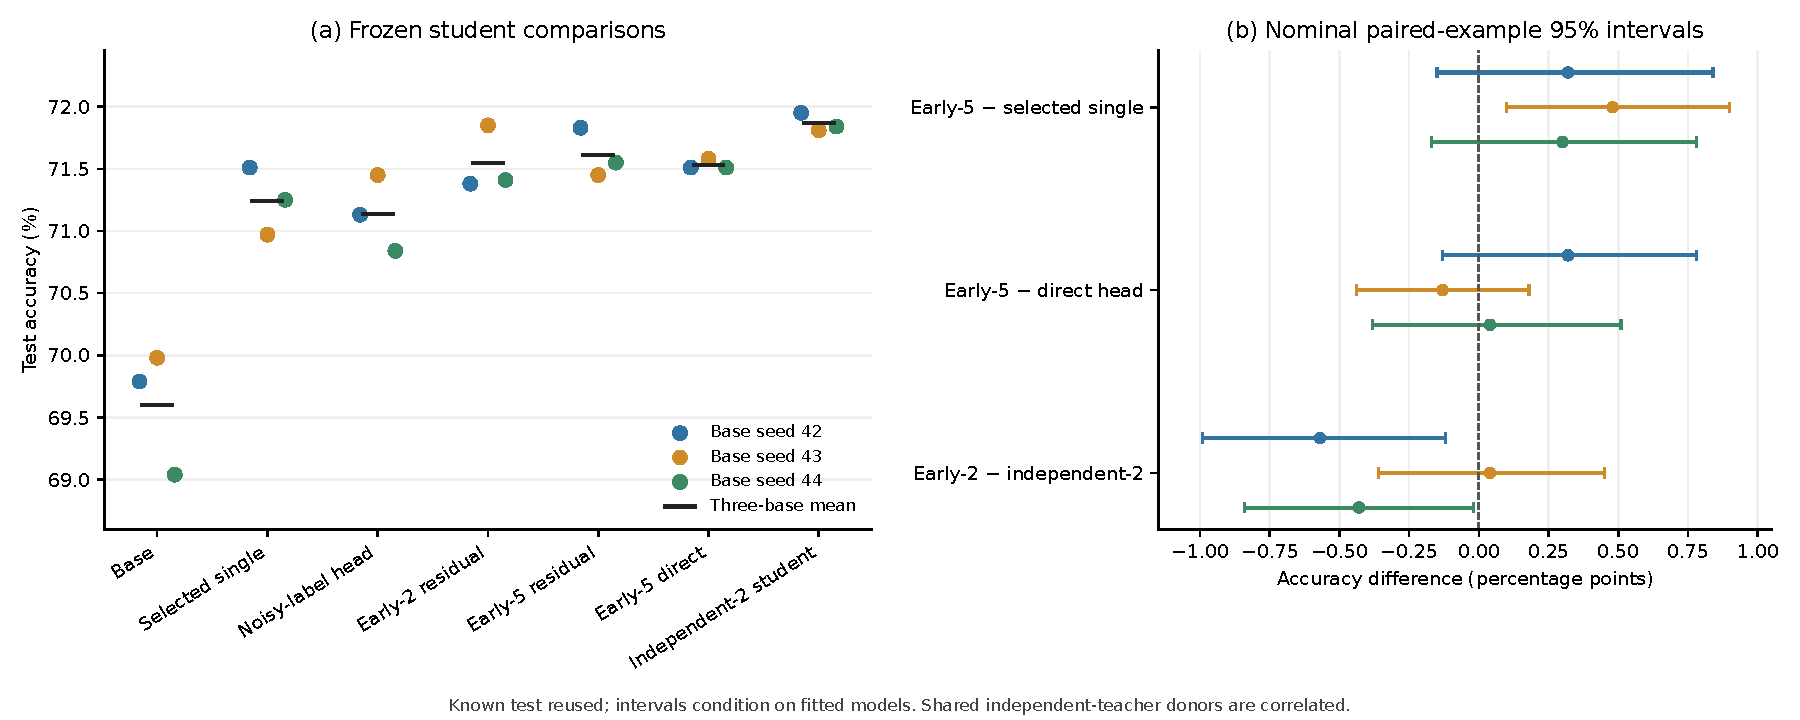
\includegraphics[width=\textwidth]{figures/posthoc_controls.pdf}
\caption{S2 frozen controls. Black marks are descriptive means over three bases.
Intervals condition on fitted models and do not quantify training-run uncertainty.}
\end{figure}

\end{document}
